% !TEX root=main.tex

\section{Discrete Kalman filter}

\subsection{5a)}

To make a discrete Kalman filter we need to discretize the model found in \cref{subsec:4a}. The discretized system can be found using the equations

\begin{subequations}
    \begin{align}
        A_d &= e^{AT_s} \\
        B_d &= \int_0^{T_s} e^{A\tau}B d\tau \\
        E_d &= \int_0^{T_s} e^{A\tau}E d\tau \\
        C_d &= C
    \end{align}
\end{subequations}

This can be done using he Matlab function \texttt{[Ad, Bd] = c2d(A, B, Ts)} to get the discretized matrices $A_d$ and $B_d$ discretized with a timestep of \texttt{Ts}. To get the model discretized with a sampling frequency of $10\si{\hertz}$ we set \texttt{Ts} to $0.1$. In order to get $E_d$ we use the same function, but swap \texttt{Bd} and \texttt{B} with \texttt{Ed} and \texttt{E}. The resulting $A_d$, $B_d$ and $E_d$ matrices are

\begin{subequations}
    \begin{align}
        A_d &= \begin{bmatrix}
        0.1000 & 0.0993 & 0 & 0 & 0 \\
        -0.0607 & 0.9841 & 0 & 0 & 0 \\
        0 & 0 & 1 & 0.0999 & -1.0063 \cdot 10^{-5} \\
        0 & 0 & 0 & 0.1000 & -0.0002 \\
        0 & 0 & 0 & 0 & 1
        \end{bmatrix} \\
        B_d &= \begin{bmatrix}
        0 \\
        0 \\
        1.0062 \cdot 10^{-5} \\
        0.0002 \\
        0
        \end{bmatrix} \\
        E_ d &= \begin{bmatrix}
        2.4880\cdot 10^{-5} & 0 \\
        0.0005 & 0 \\
        0 & -3.3545\cdot 10^{-7} \\
        0 & -1.0063\cdot 10^{-5} \\
        0 & 0.1000
        \end{bmatrix}
    \end{align}
\end{subequations}

\subsection{5b)}

Another thing we need to make a Kalman filter is the variance of the measurement noise. The variance was found by simulating long timeseries of the ship with a input of zero, and with measurement noise turned on. The variance was found using the Matlab function \texttt{ts\_var = var(ts)}, where \texttt{ts} is a timeseries, and \texttt{ts\_var} is the variance of the timeseries. The variance of the measurement noise was found to be $0.002$. However this is in degrees squared, whereas we want the variance in radians (squared). This gives us a variance of $6.0923 \cdot 10^{-6}$.

\subsection{5c)}

% Update step
%K = P_est_pre*transpose(Cd)/(Cd*P_est_pre*transpose(Cd) + R);
%x_est = x_est_pre + K * (psi_meas - Cd*x_est_pre);
%P_est = (eye(5)-K*Cd)*P_est_pre*transpose(eye(5)-K*Cd) + K*R*transpose(K);

A Kalman filter was implemented using Simulink with a Matlab function block. The custom Kalman filter subsystems structure is shown in \cref{fig:kalman_subsys}. The rudder angle and measured compass angle are converted to radians, discretized by a zero-order hold block, and passed into the Kalman filter function. The estimated state from the filter is passed through a memory block to avoid an algebraic loop, converted back to degrees, and finally split up to expose the different states.

The Kalman filter function itself is listed in \cref{lst:kalman}. The first time the function is called, it initializes the a priori states to the provided values. After that, it calculates the Kalman gain, state estimate and covariance estimate using the update equations

\begin{subequations}
    \begin{align}
        K_k &= P_k^-C_d^T(C_dP_k^-C_d^T+R)^{-1} \\
        \hat{x}_k &= \hat{x}_k^- + K_k(y_k - C_d\hat{x}_k^-) \\
        P_k &= (I - K_kC_d)P_k^-(I-K_kC_d) + K_kRK_k^T
    \end{align}

\end{subequations}

%% Projection step
%x_est_pre = Ad*x_est + Bd*delta;
%P_est_pre = Ad*P_est*transpose(Ad) + Ed*Q*transpose(Ed);

and finally updates the a priori estimates using the prediction equations

\begin{subequations}
    \begin{align}
        \hat{x}_{k+1}^- &= A_d\hat{x}_k \\
        P_{k+1}^- &= A_d P_k A_d^T + E_d Q E_d^T
    \end{align}

\end{subequations}

\lstinputlisting[language=Matlab, basicstyle=\small, caption={Matlab implementation of the discrete Kalman filter}, label={lst:kalman},float]{listings/kalman.m}

\begin{figure}
    \centering
    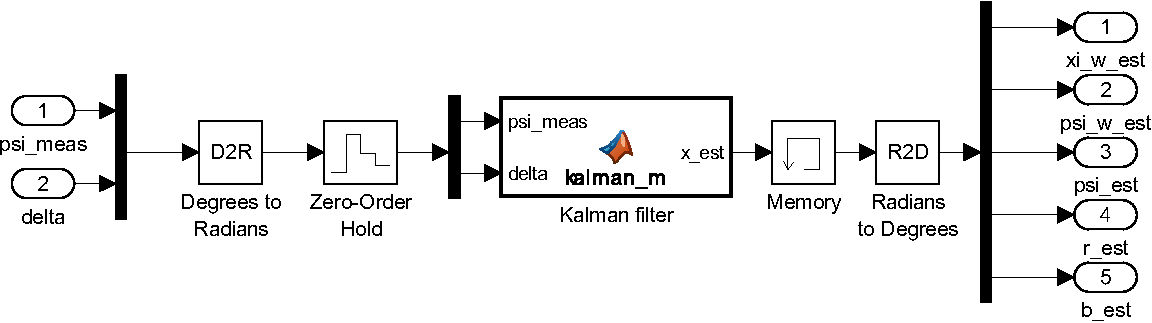
\includegraphics[width=\textwidth]{images/oppg5/c_kalman.pdf}
    \caption{Implementation of the Kalman filter subsystem in Simulink.}
    \label{fig:kalman_subsys}
\end{figure}

\subsection{5d)}

\begin{figure}
    \centering
    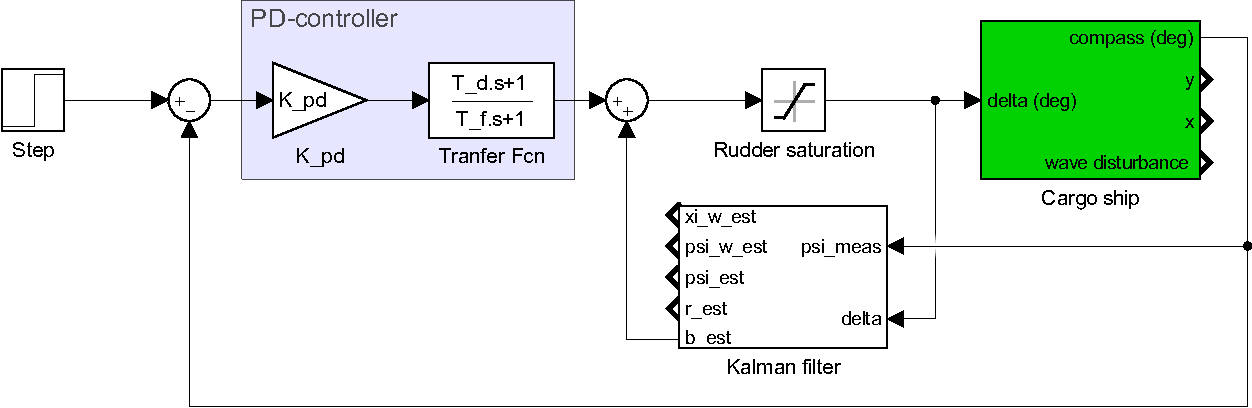
\includegraphics[width=\textwidth]{images/oppg5/bias_FF.pdf}
    \caption{Simulink implementation of PD control with estimated bias feed forward.}
    \label{fig:bias_ff}
\end{figure}

\begin{figure}
    \centering
    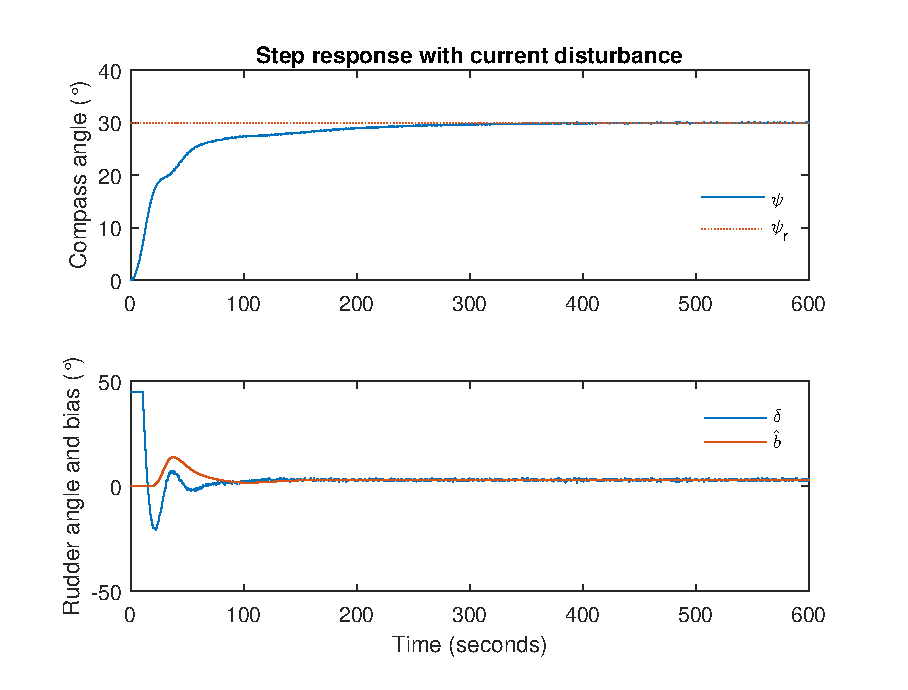
\includegraphics[width=\textwidth]{images/oppg5/5d.eps}
    \caption{Simulation results with estimated bias feed-forward.}
    \label{fig:5d}
\end{figure}


\subsection{5e)}

\begin{figure}
    \centering
    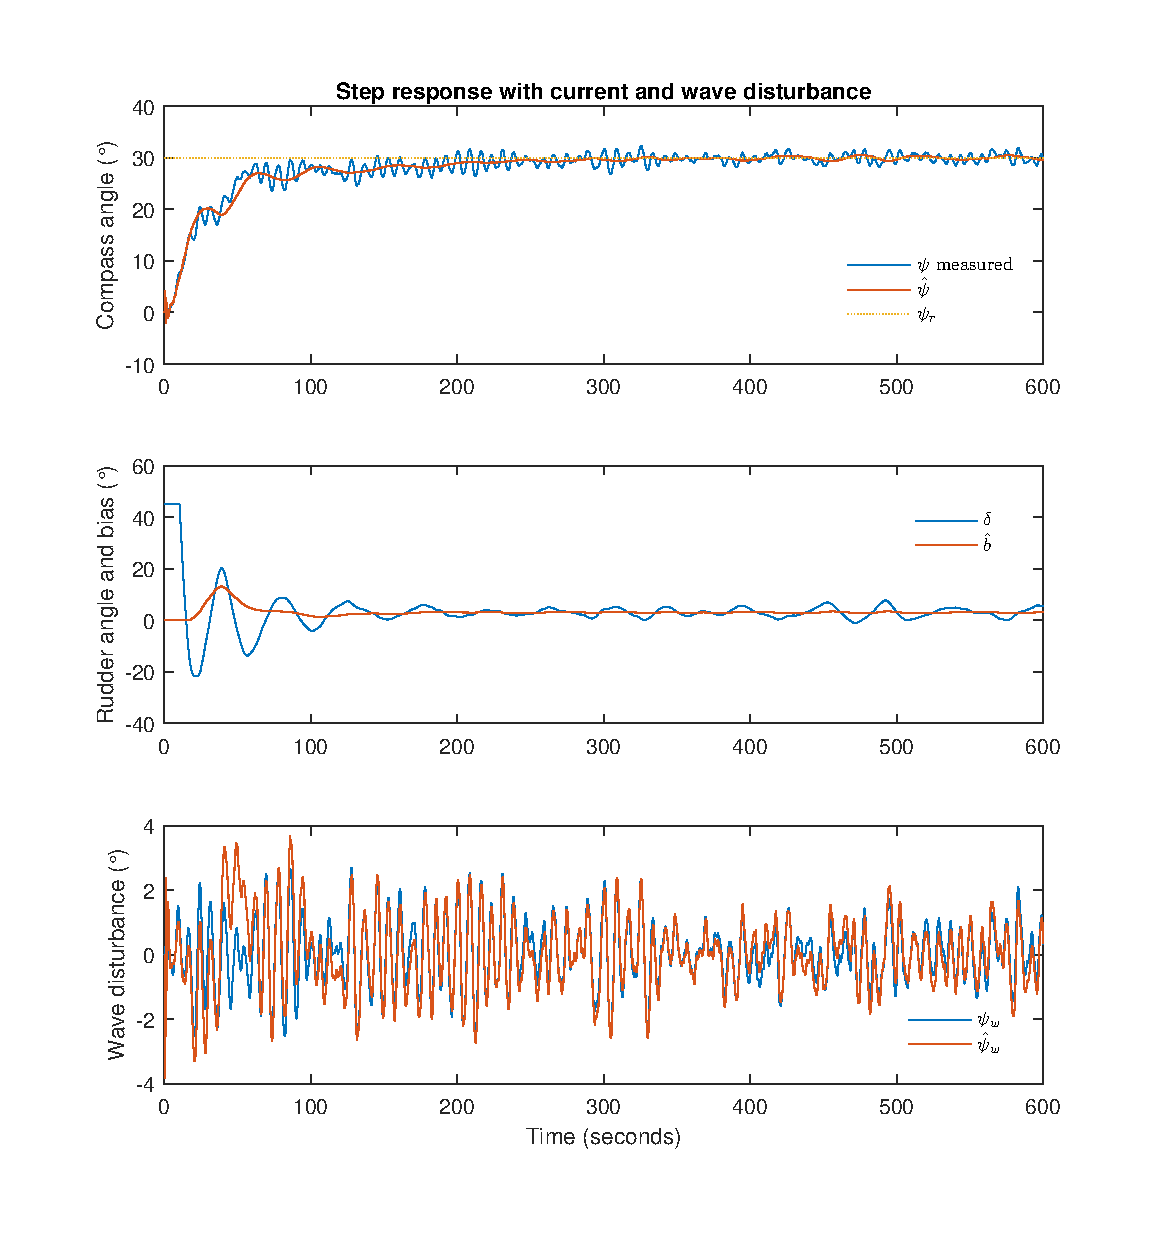
\includegraphics[width=\textwidth]{images/oppg5/5e.eps}
    \caption{Simulation results with estimated bias feed-forward and wave-filtered feedback}
    \label{fig:5e}
\end{figure}

\begin{figure}
    \centering
    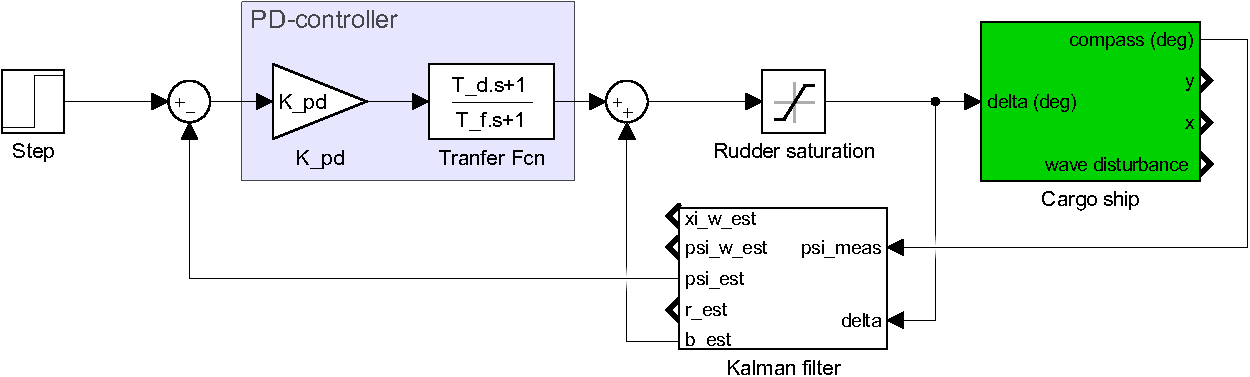
\includegraphics[width=\textwidth]{images/oppg5/bias_FF_and_filtered_FB.pdf}
    \caption{Simulink implementation of PD control with estimated bias feed forward, and filtered feedback.}
    \label{fig:filtered_fb}
\end{figure}
